\documentclass{article}
\usepackage{graphicx}

\begin{document}

\title{CSE 6220 PA 1}
\author{Karl Hiner, Harshit Srivastava, Dalton Yu}
\maketitle

Below is a chart showing the execution time of the program (in seconds) vs. the number of processors for $p = [1,2,..., 24]$.
This experiment was performed on the COC-ICE cluster.

\begin{figure}[htb]
    \centering 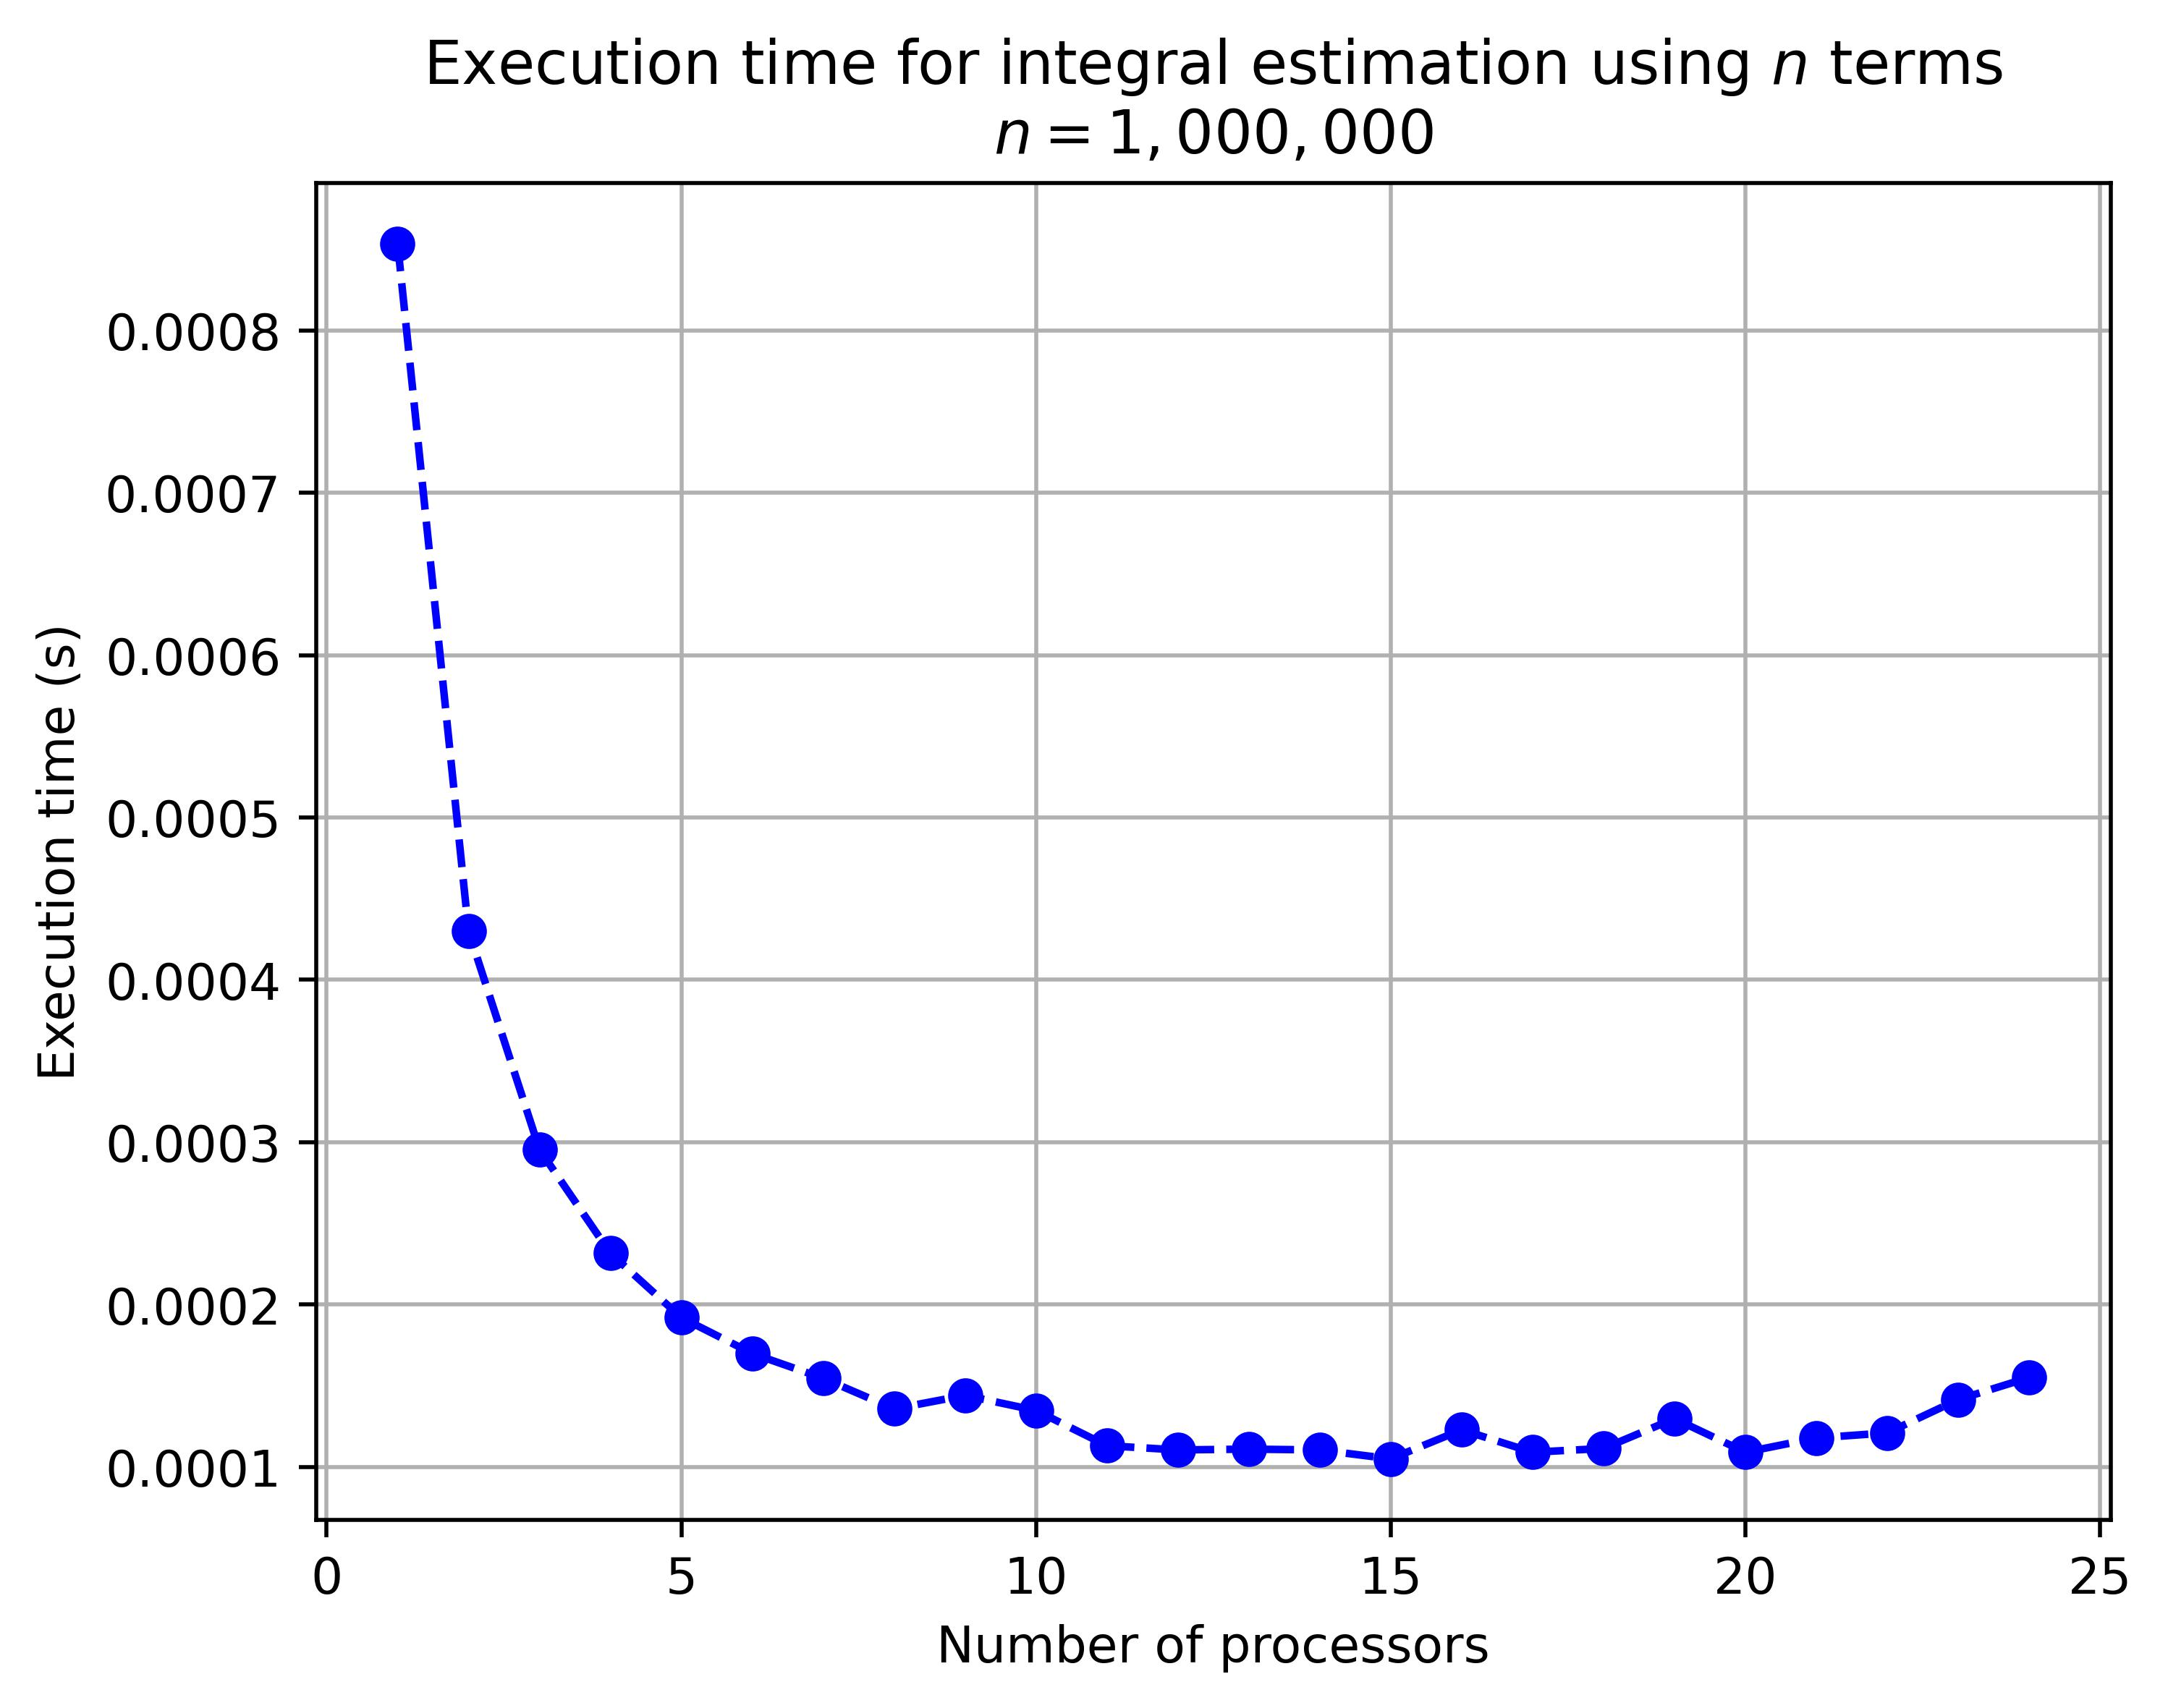
\includegraphics[scale = 0.75]{report_chart_n_1M_PACE.jpg}
    \caption{$n=10^6$, $p=[1,2,...,24]$ on PACE cluster}
    \label{fig:figure1}
\end{figure}

Note that this chart evaluates every value of $p$ in the tested range.
Since the problem does not require a substantial chunk of memory for running the evaluation, the computational bottleneck shifts to the CPU cores and Interconnect Network-on-Chip (NoC) used by these cores to communicate with each other. The execution time for $p = 2$ is very nearly half that of $p = 1$, showing a near-ideal speedup. Likewise, $p = 4$ shows roughly a 2X speedup over $p = 2$, as expected for this embarrassingly parallel algorithm.

However, these speedups gradually decrease as we add processors, reaching a minimum somewhere in the range $p \in [14, 20]$, and execution times even begin to consistently climb back up as $p > 20$.
This is because, while the problem size dedicated to each CPU core decreases, the Interconnect NoC traffic increases, making it the bottleneck in the overall computation.

Note that with a problem size of $n=10^6$, using $p=20$ processors results in each process is responsible for $\frac{10^6}{20} = 5\cdot 10^4$ summation terms.
Calculating each term involves three multiplications and two additions for a total of five operations each.
Thus, we see Interconnect NoC communication overhead dominating the runtime when each processor is responsible for roughly $\leq \frac{1}{4}$M double-precision floating point operations.

\hbox{}
Note that we cap our processor count at $p=24$ since this experiment was run on the COC-ICE cluster, which has 24 cores per node. Intel's server-grade computers use Compute eXpress Link(CXL) Bus (an advanced version of PCI express BUS interface) for communicating with other CPU nodes. 
Thus, when $p>24$, we encounter dramatically higher execution times, due to the CXL bus communication latency, which is much higher than Interconnect NoC communication delay.

This is clear from the following chart, which shows execution times for  $p=[1,2,...,48]$:

\begin{figure}[htb]
    \centering 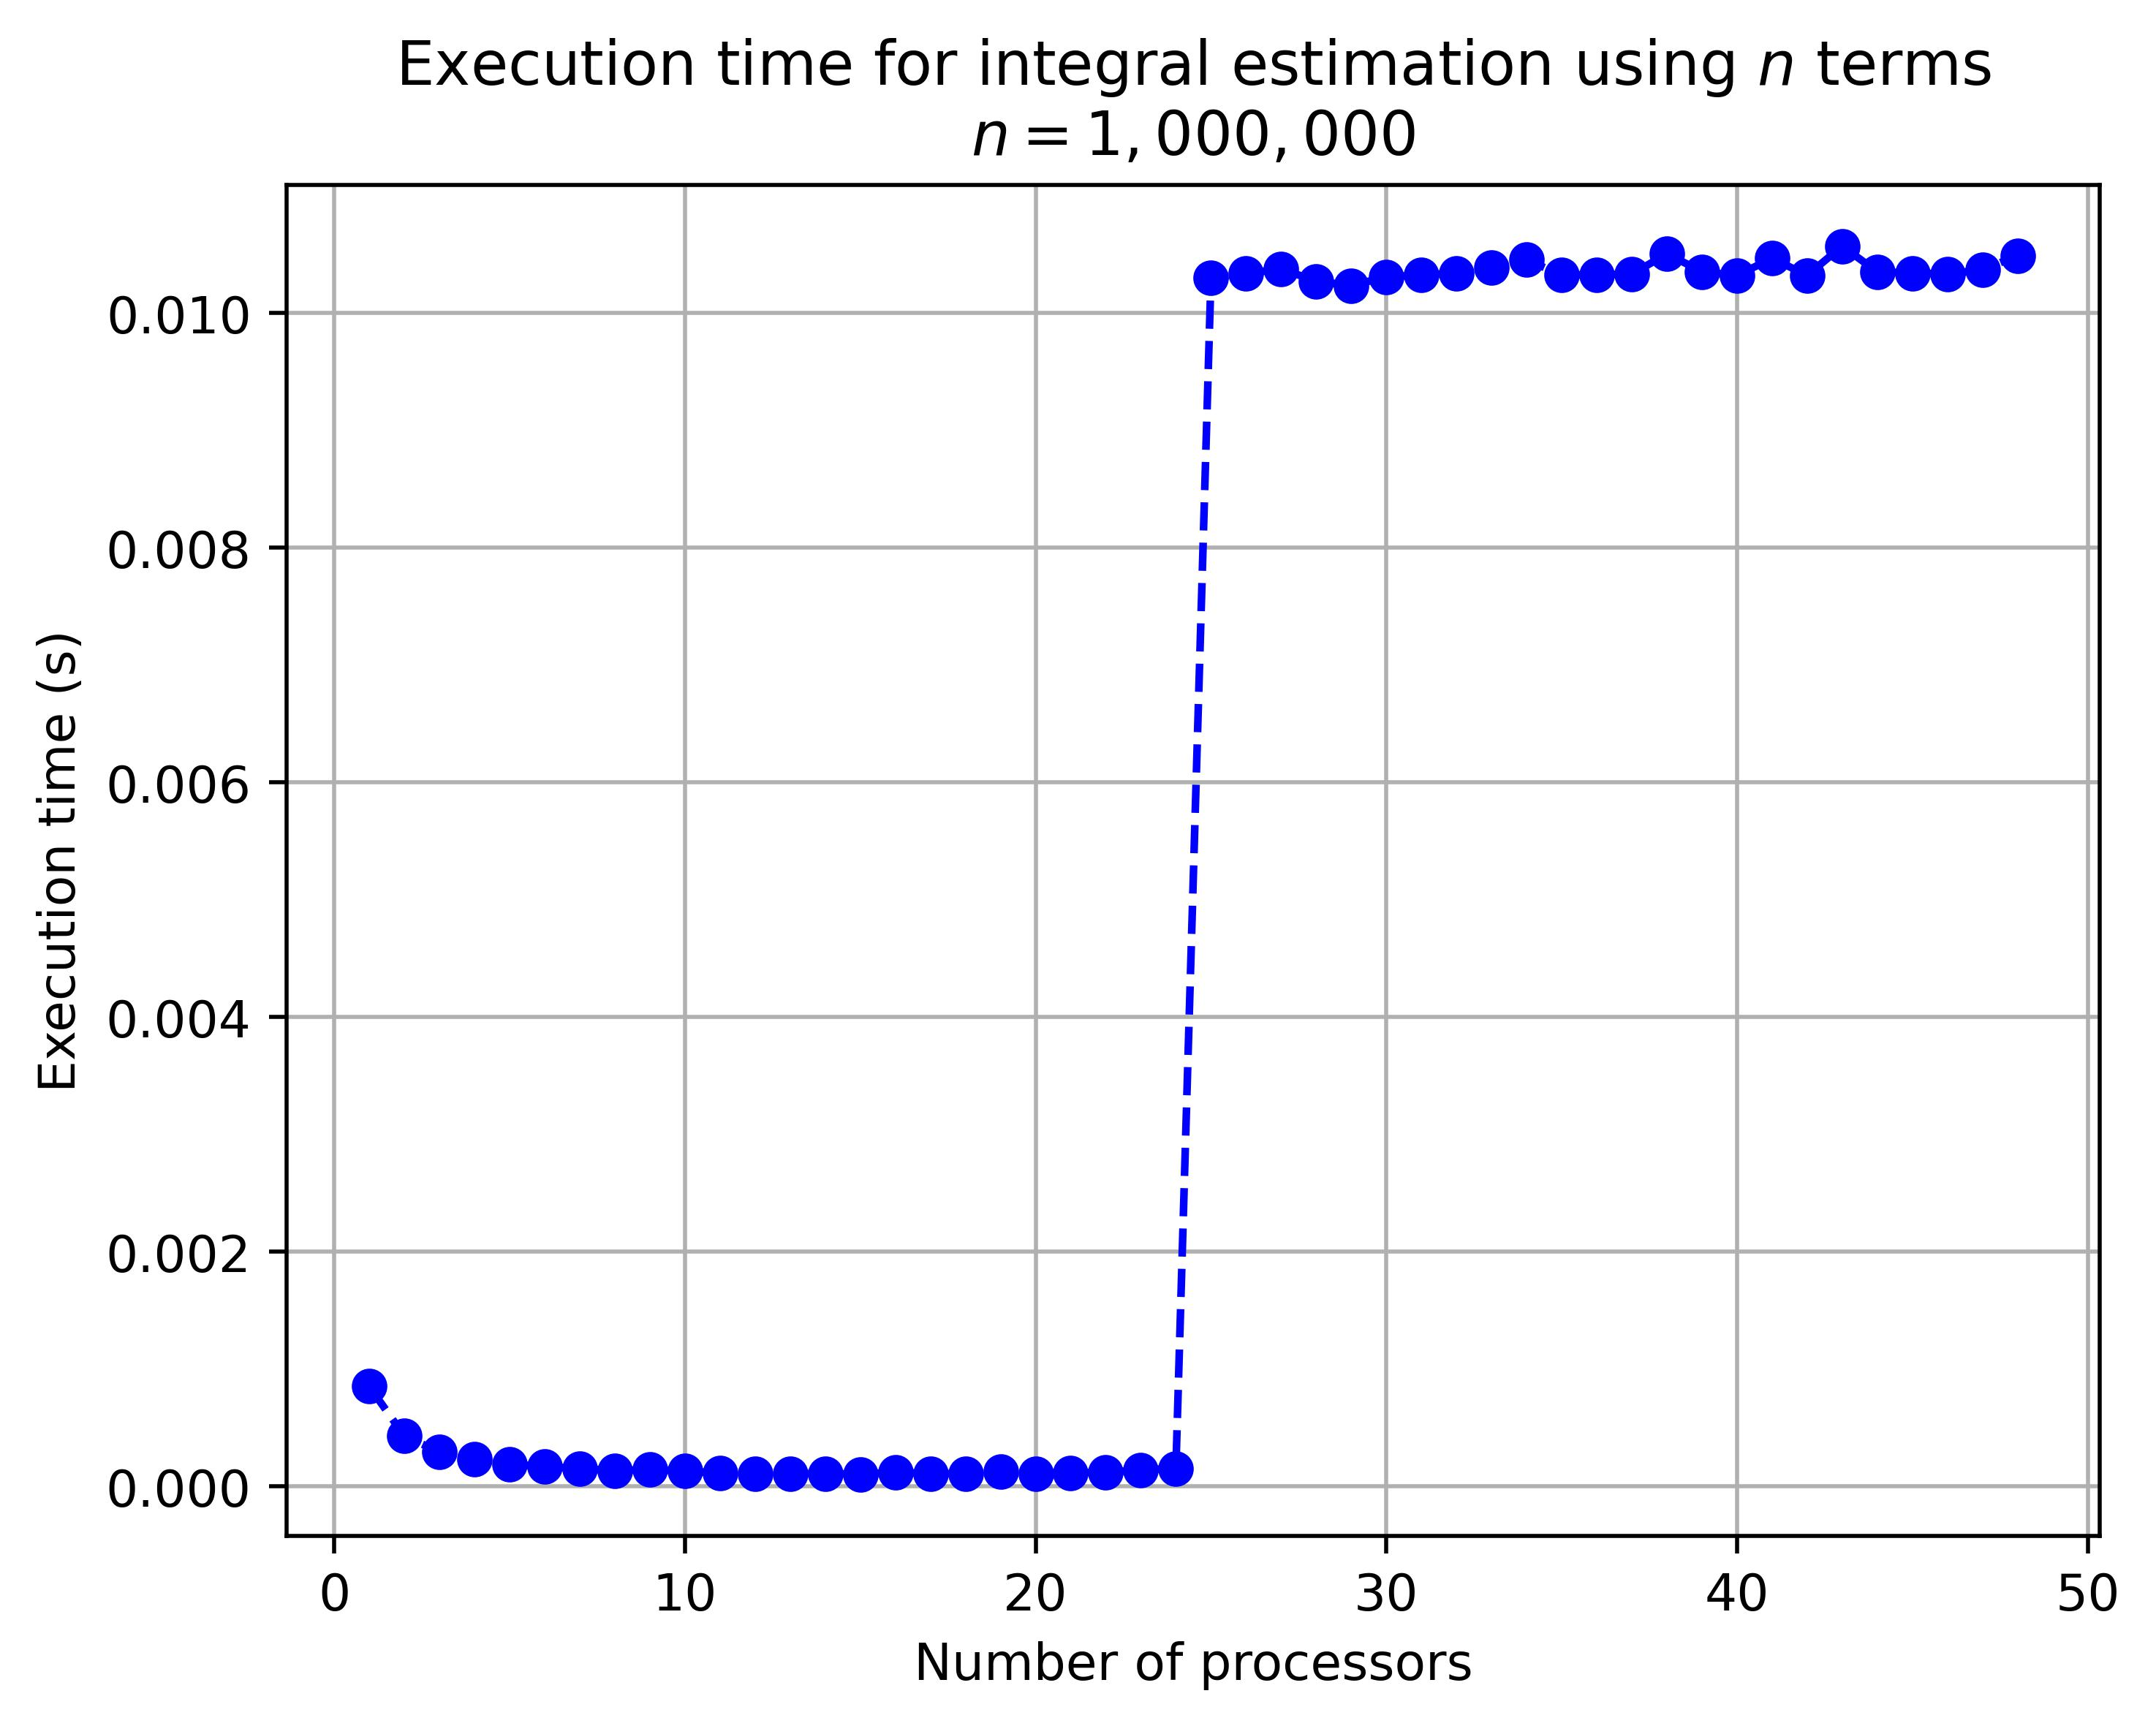
\includegraphics[scale = 0.75]{report_chart_n_1M_p_48_PACE.jpg}
    \caption{$n=10^6$, $p=[1,2,...,48]$ on PACE cluster}
    \label{fig:figure2}
\end{figure}

\end{document}
